
\documentclass[twoside]{article}
\setlength{\oddsidemargin}{0.25 in}
\setlength{\evensidemargin}{-0.25 in}
\setlength{\topmargin}{-0.6 in}
\setlength{\textwidth}{6.5 in}
\setlength{\textheight}{8.5 in}
\setlength{\headsep}{0.75 in}
\setlength{\parindent}{0 in}
\setlength{\parskip}{0.1 in}

\usepackage{amsmath,amsfonts,graphicx}

\usepackage{color}
\usepackage{mathtools}

\usepackage{subcaption} 
\usepackage{subfig}

\usepackage{float}
\usepackage{listings}
\usepackage[svgnames]{xcolor}
\definecolor{mygray}{rgb}{0.9,0.9,0.9}
\lstset{language=R,
	basicstyle=\small\ttfamily,
	stringstyle=\color{DarkGreen},
	otherkeywords={0,1,2,3,4,5,6,7,8,9},
	morekeywords={TRUE,FALSE},
	deletekeywords={data,frame,length,as,character},
	keywordstyle=\color{blue},
	commentstyle=\color{DarkGreen},
	frame=single,
	backgroundcolor=\color{mygray},
	numbers=left, 
}
%
% The following commands set up the lecnum (chap number)
% counter and make various numbering schemes work relative
% to the chap number.
%
\newcounter{lecnum}
\renewcommand{\thepage}{\thelecnum-\arabic{page}}
\renewcommand{\thesection}{\thelecnum.\arabic{section}}
\renewcommand{\theequation}{\thelecnum.\arabic{equation}}
\renewcommand{\thefigure}{\thelecnum.\arabic{figure}}
\renewcommand{\thetable}{\thelecnum.\arabic{table}}

%
% The following macro is used to generate the header.
%
\newcommand{\chap}[4]{
   \pagestyle{myheadings}
   \thispagestyle{plain}
   \newpage
   \setcounter{lecnum}{#1}
   \setcounter{page}{1}
   \noindent
   \begin{center}
   \framebox{
      \vbox{\vspace{2mm}
    \hbox to 6.28in { {\bf SDS 383D: Modeling II
	\hfill Spring 2017} }
       \vspace{4mm}
       \hbox to 6.28in { {\Large \hfill Section #1: #2  \hfill} }
       \hbox to 6.28in { { \hfill Student: Natalia Zuniga-Garcia  \hfill} }
      \vspace{2mm}}
   }
   \end{center}
   \markboth{Section #1: #2}{Section #1: #2}

   
}
%
% Convention for citations is authors' initials followed by the year.
% For example, to cite a paper by Leighton and Maggs you would type
% \cite{LM89}, and to cite a paper by Strassen you would type \cite{S69}.
% (To avoid bibliography problems, for now we redefine the \cite command.)
% Also commands that create a suitable format for the reference list.
%\renewcommand{\cite}[1]{[#1]}
%\def\beginrefs{\begin{list}%
%        {[\arabic{equation}]}{\usecounter{equation}
%         \setlength{\leftmargin}{2.0truecm}\setlength{\labelsep}{0.4truecm}%
%         \setlength{\labelwidth}{1.6truecm}}}
%\def\endrefs{\end{list}}
%\def\bibentry#1{\item[\hbox{[#1]}]}

%Use this command for a figure; it puts a figure in wherever you want it.
%usage: \fig{NUMBER}{SPACE-IN-INCHES}{CAPTION}
\newcommand{\fig}[3]{
			\vspace{#2}
			\begin{center}
			Figure \thelecnum.#1:~#3
			\end{center}
	}
% Use these for theorems, lemmas, proofs, etc.
\newtheorem{theorem}{Theorem}[lecnum]
\newtheorem{lemma}[theorem]{Lemma}
\newtheorem{proposition}[theorem]{Proposition}
\newtheorem{claim}[theorem]{Claim}
\newtheorem{corollary}[theorem]{Corollary}
\newtheorem{definition}[theorem]{Definition}
\newtheorem{exercise}{Exercise}[lecnum]
\newtheorem{example}{Example}[lecnum]
\newenvironment{proof}{{\bf Proof:}}{\hfill\rule{2mm}{2mm}}

% **** IF YOU WANT TO DEFINE ADDITIONAL MACROS FOR YOURSELF, PUT THEM HERE:

\newcommand\E{\mathbb{E}}
\newcommand\Prob{\mathbf{P}}
\newcommand\Q{\mathbf{Q}}
\newcommand\cov{\mbox{cov}}
\begin{document}
\chap{2}{Bayesian inference in Gaussian models}
\maketitle

\section{Bayesian inference in a simple Gaussian model}

Let's start with a simple, one-dimensional Gaussian example, where

$$y_i |\mu, \sigma^2 \sim \mbox{N}(\mu,\sigma^2).$$

We will assume that $\mu$ and $\sigma$ are unknown, and will put conjugate priors on them both, so that
$$\begin{aligned}
  \sigma^2 \sim& \mbox{Inv-Gamma}(\alpha_0, \beta_0)\\
  \mu|\sigma^2 \sim& \mbox{Normal}\left(\mu_0, \frac{\sigma^2}{\kappa_0}\right)\end{aligned}$$

or, equivalently,
$$\begin{aligned}
  y_i |\mu, \omega \sim& \mbox{N}(\mu,1/\omega)\\
  \omega \sim& \mbox{Gamma}(\alpha_0, \beta_0)\\
  \mu|\omega \sim& \mbox{Normal}\left(\mu_0, \frac{1}{\omega\kappa_0}\right)\end{aligned}$$

We refer to this as a normal/inverse gamma prior on $\mu$ and $\sigma^2$ (or a normal/gamma prior on $\mu$ and $\omega$). We will now explore the posterior distributions on $\mu$ and $\omega$(/$\sigma^2$) -- much of this will involve similar results to those obtained in the first set of exercises.




\begin{exercise}
  Derive the conditional posterior distributions $p(\mu, \omega|y_1,\dots, y_n)$ (or $p(\mu, \sigma^2|y_1,\dots, y_n)$) and show that it is in the same family as $p(\mu, \omega)$. What are the updated parameters $\alpha_n, \beta_n,\mu_n$ and $\kappa_n$?
\end{exercise}

\color{blue}
\textbf{Solution}

We know that,
$$ p(\mu, \omega|y_i) \propto p(y_i|\mu, \omega) p(\mu, \omega) $$
First, we find the likelihood $ p(y_i|\mu, \omega)$,
$$  p(y_i|\mu, \omega) = \bigg(\frac{\omega}{ 2 \pi} \bigg)^{\frac{n}{2}} \exp\left\{ -\frac{\omega}{2} \sum_{i=1}^{n} (y_i - \mu)^2 
\right\}  
$$
Now we find the prior $p(\mu, \omega)$,
$$p(\mu, \omega) = p(\mu | \omega) p(\omega)  $$
Where,
$$ p(\mu | \omega) = \bigg(\frac{\omega \kappa_0}{ 2 \pi} \bigg)^{\frac{1}{2}} \exp\left\{ -\frac{\omega \kappa_0}{2} (\mu - \mu_0)^2 \right\}  $$
$$p(\omega) = \frac{\beta_0^{\alpha_0}}{\Gamma (\alpha_0) }\omega^{\alpha_0-1} exp\{-\beta_0 \omega\}$$
Therefore we have,
$$p(\mu, \omega) = 
\bigg(\frac{\omega \kappa_0}{ 2 \pi} \bigg)^{\frac{1}{2}} \exp\left\{ -\frac{\omega \kappa_0}{2} (\mu - \mu_0)^2 \right\} 
\frac{\beta_0^{\alpha_0}}{\Gamma (\alpha_0) }\omega^{\alpha_0-1} exp\{-\beta_0 \omega\}$$
$$
= \bigg(\frac{\kappa_0}{ 2 \pi} \bigg)^{\frac{1}{2}} \frac{\beta_0^{\alpha_0}}{\Gamma (\alpha_0) }\
 \omega^{\alpha_0-\frac{1}{2}} 
\exp\left\{ -\frac{\omega }{2} [\kappa_0(\mu - \mu_0)^2 + 2\beta_0] \right\} 
$$
$$\propto \mbox{NG}(\mu_0, \kappa_0, \alpha_0, \beta_0)$$

Now we can estimate the posterior,
$$ p(\mu, \omega|y_i) \propto p(y_i|\mu, \omega) p(\mu, \omega) $$
$$ \propto  \omega^{\frac{n}{2}} \exp\left\{ -\frac{\omega}{2} \sum_{i=1}^{n} (y_i - \mu)^2 \right\} 
 \omega^{\alpha_0-\frac{1}{2}} 
\exp\left\{ -\frac{\omega }{2} [\kappa_0(\mu - \mu_0)^2 + 2\beta_0] \right\} $$
$$  \propto \omega^{\frac{1}{2}}  \omega^{\alpha_0 + \frac{n}{2}-1 } 
\exp\left\{ -\beta_0 \gamma \right\} 
\exp\left\{ -\frac{\omega}{2} [ \kappa_0(\mu - \mu_0)^2 + \sum_{i=1}^{n} (y_i - \mu)^2 ] \right\} 
$$
Where,
$$ \sum_{i=1}^{n} (y_i - \mu)^2 = \sum_{i=1}^{n} [(y_i - \overline{y} )^2 - (\mu - \overline{y})^2 ] = n(\mu - \overline{y})^2+ \sum_{i=1}^{n} (y_i - \overline{y})^2
$$
and,
$$ 
 \kappa_0(\mu - \mu_0)^2  + n(\mu - \overline{y})^2 = 
 ( \kappa_0 + n)\bigg( \mu - \frac{\kappa_0 \mu_0 + n\overline{y}}{\kappa_0 + n} \bigg)^2+
 \frac{\kappa_0 n (\overline{y}-\mu_0)^2}{\kappa_0+n}
$$
Then we have that,
$$\kappa_0(\mu - \mu_0)^2 + \sum_{i=1}^{n} (y_i - \mu)^2 
= (\kappa_0 + n) \bigg( \mu - \frac{\kappa_0 \mu_0 + n\overline{y}}{\kappa_0 + n} \bigg)^2
+ \frac{\kappa_0 n (\overline{y}-\mu_0)^2}{\kappa_0+n} + \sum_{i=1}^{n} (y_i - \overline{y})^2 $$
Now going back to the posterior,
$$ p(\mu, \omega|y_i) \propto  \omega^{\frac{1}{2}}  \omega^{\alpha_0 + \frac{n}{2}-1 } 
\exp\left\{ -\beta_0 \omega \right\} 
\exp\left\{ -\frac{1}{2} [ \kappa_0(\mu - \mu_0)^2 + \sum_{i=1}^{n} (y_i - \mu)^2 ] \right\} $$ $$
\propto  \omega^{\frac{1}{2}}  \omega^{\alpha_0 + \frac{n}{2}-1 } 
\exp\left\{ -\beta_0 \omega \right\} 
\exp\left\{ -\frac{\omega}{2} \bigg[  (\kappa_0 + n) \bigg( \mu - \frac{\kappa_0 \mu_0 + n\overline{y}}{\kappa_0 + n} \bigg)^2 +
\frac{\kappa_0 n (\overline{y}-\mu_0)^2}{\kappa_0+n} + \sum_{i=1}^{n} (y_i - \overline{y})^2 \bigg] \right\} $$
$$ \propto
\omega^{\frac{1}{2}} \exp\left\{ -\frac{\omega}{2}  (\kappa_0 + n)  \bigg( \mu - \frac{\kappa_0 \mu_0 + n\overline{y}}{\kappa_0 + n} \bigg)^2 \right\} 
\omega^{\alpha_0 + \frac{n}{2}-1 } \exp\left\{ -\beta_0 \omega
 -\frac{\omega}{2} \bigg[
\frac{\kappa_0 n (\overline{y}-\mu_0)^2}{\kappa_0+n} + \sum_{i=1}^{n} (y_i - \overline{y})^2 \bigg]
\right\} 
$$
$$ \propto
\mbox{Normal}\left( \frac{\kappa_0 \mu_0 + n\overline{y}}{\kappa_0 + n},  \frac{1}{\omega(\kappa_0 + n)}
\right) 
\mbox{Gamma}\bigg(\alpha_0 + \frac{n}{2}, \beta_0 + \frac{1}{2} \bigg[
\frac{\kappa_0 n (\overline{y}-\mu_0)^2}{\kappa_0+n} + \sum_{i=1}^{n} (y_i - \overline{y})^2 \bigg] \bigg)
$$
$$\propto \mbox{NG}(\mu_n, \kappa_n, \alpha_n, \beta_n)$$
Thus, the updated parameters are:
\begin{itemize}
	\item  $\alpha_n = \alpha_0 + \frac{n}{2} $
	\item $ \beta_n = \beta_0 + \frac{1}{2} \bigg[
	\frac{\kappa_0 n (\overline{y}-\mu_0)^2}{\kappa_0+n} + \sum_{i=1}^{n} (y_i - \overline{y})^2 \bigg]  $
	\item $ \mu_n =  \frac{\kappa_0 \mu_0 + n\overline{y}}{\kappa_0 + n}$ 
	\item $ \kappa_n = \kappa_0 + n$
\end{itemize}



\color{black}

\begin{exercise}
  Derive the conditional posterior distribution $p(\mu|\omega,y_1,\dots, y_n)$ and $p(\omega|y_1,\dots, y_n)$ (or if you'd prefer, $p(\mu|\sigma^2, y_1,\dots, y_n)$ and $p(\sigma^2|y_1,\dots, y_n)$). Based on this and the previous exercise, what are reasonable interpretations for the parameters $\mu_0,\kappa_0, \alpha_0$ and $\beta_0$?
\end{exercise}


\color{blue}
\textbf{Solution}

We know that,
$$ p(\mu|\omega,y_i) \propto  p(y_i |\mu,\omega) p(\mu|\omega)  $$
Where,
$$ p(\mu | \omega) = \bigg(\frac{\omega \kappa_0}{ 2 \pi} \bigg)^{\frac{1}{2}} \exp\left\{ -\frac{\omega \kappa_0}{2} (\mu - \mu_0)^2 \right\}  $$
$$  p(y_i|\mu, \omega) = \bigg(\frac{\omega}{ 2 \pi} \bigg)^{\frac{n}{2}} \exp\left\{ -\frac{\omega}{2} \sum_{i=1}^{n} (y_i - \mu)^2 
\right\}  $$
Then,
$$ p(\mu|\omega,y_i)  \propto 
 \bigg(\frac{\omega}{ 2 \pi} \bigg)^{\frac{n}{2}} \exp\left\{ -\frac{\omega}{2} \sum_{i=1}^{n} (y_i - \mu)^2 \right\} 
\bigg(\frac{\omega \kappa_0}{ 2 \pi} \bigg)^{\frac{1}{2}} \exp\left\{ -\frac{\omega \kappa_0}{2} (\mu - \mu_0)^2 \right\} $$
$$ \propto \exp\left\{ -\frac{\omega }{2}[ \kappa_0 (\mu - \mu_0)^2 + \sum_{i=1}^{n} (y_i - \mu)^2 ] \right\} 
\propto \exp\left\{ -\frac{\omega}{2}  (\kappa_0 + n)  \bigg( \mu - \frac{\kappa_0 \mu_0 + n\overline{y}}{\kappa_0 + n} \bigg)^2 \ \right\} $$
$$ \propto
\mbox{Normal}\left( \frac{\kappa_0 \mu_0 + n\overline{y}}{\kappa_0 + n},  \frac{1}{\omega(\kappa_0 + n)}
\right)  $$

Now for $\omega$ we have,
$$ p(\omega|y_i) \propto p(y_i|\mu, \omega) p(\omega) $$
Where,
$$p(\omega) = \frac{\beta_0^{\alpha_0}}{\Gamma (\alpha_0) }\omega^{\alpha_0-1} exp\{-\beta_0 \omega\}$$
Then,
$$p(\omega|y_i)  \propto \bigg(\frac{\omega}{ 2 \pi} \bigg)^{\frac{n}{2}} \exp\left\{ -\frac{\omega}{2} \sum_{i=1}^{n} (y_i - \mu)^2 
\right\} \frac{\beta_0^{\alpha_0}}{\Gamma (\alpha_0) }\omega^{\alpha_0-1} exp\{-\beta_0 \omega\} $$
$$\propto  \exp\left\{ -\beta_0 \omega
-\frac{\omega}{2} \bigg[
\frac{\kappa_0 n (\overline{y}-\mu_0)^2}{\kappa_0+n} + \sum_{i=1}^{n} (y_i - \overline{y})^2 \bigg]
\right\}  $$
$$ \propto \mbox{Gamma}\bigg(\alpha_0 + \frac{n}{2}, \beta_0 + \frac{1}{2} \bigg[
\frac{\kappa_0 n (\overline{y}-\mu_0)^2}{\kappa_0+n} + \sum_{i=1}^{n} (y_i - \overline{y})^2 \bigg] \bigg)
$$

What are reasonable interpretations for the parameters $\mu_0,\kappa_0, \alpha_0$ and $\beta_0$?

\begin{itemize}
	\item $\kappa_0$ is the "prior sample size" for $\mu$.
	\item $\mu_0$ is the prior guest on $\mu$ and $\mu_n$ is the posterior of $\mu$ that we can see is a weighted average based on the sample size $n$ and the "prior sample size" $\kappa_0$.
	\item $\alpha_0$ is the "prior sample size" for the error variance $\sigma^2$.
	\item $\beta_0$ is the "prior sum of squares" for the error variance $\sigma^2$. For the posterior, we have $\beta_n$ which combines the "prior sum of squares" $\beta_0$, the sample sum of squares $\sum_{i=1}^{n} (y_i - \overline{y})^2$, and a term due to the discrepancy between the prior mean and the sample mean.
\end{itemize}
\color{black}

\begin{exercise}
  Show that the marginal distribution over $\mu$ is a centered, scaled $t$-distribution (note we showed something very similar in the last set of exercises!), i.e.\
  $$p(\mu) \propto \left(1+\frac{1}{\nu}\frac{(\mu-m)^2}{s^2}\right)^{-\frac{\nu+1}{2}}$$
  What are the location parameter $m$, scale parameter $s$, and degree of freedom $\nu$?
\end{exercise}

\color{blue}
\textbf{Solution}

We can compute the marginal as follow,
$$ p(\mu) \propto \int_{0}^{\infty } p(\mu, \omega) d\omega 
$$
Where, 
$$p(\mu, \omega) 
= \bigg(\frac{\kappa_0}{ 2 \pi} \bigg)^{\frac{1}{2}} \frac{\beta_0^{\alpha_0}}{\Gamma (\alpha_0) }\
\omega^{\alpha_0-\frac{1}{2}} 
\exp\left\{ -\frac{\omega }{2} [\kappa_0(\mu - \mu_0)^2 + 2\beta_0] \right\} 
$$
Then, 
$$ p(\mu) \propto  \int_{0}^{\infty } 
\omega^{\alpha_0+\frac{1}{2}-1} 
\exp\left\{ -\frac{\omega }{2} [\kappa_0(\mu - \mu_0)^2 + 2\beta_0] \right\} 
d\omega
$$
Which is the kernel of a $\mbox{Gamma}\bigg(\alpha_0 + \frac{1}{2}, 
\beta_0 + \frac{\kappa_0(\mu - \mu_0)^2}{2} \bigg) $. Then, we have that the normalization constant of the distribution is,

$$ p(\mu) \propto 
\frac{\Gamma(\alpha_0 + \frac{1}{2}) }{[\beta_0 + \frac{\kappa_0(\mu - \mu_0)^2}{2}]^{\alpha_0 + \frac{1}{2}}}$$ 
$$  \propto 
\bigg[\beta_0 + \frac{\kappa_0(\mu - \mu_0)^2}{2}\bigg]^{-\alpha_0 - \frac{1}{2}}$$
$$  \propto 
\bigg[1 + \frac{1}{2\alpha_0}\frac{\alpha_0\kappa_0(\mu - \mu_0)^2}{\beta_0}\bigg]^{-\frac{(2\alpha_0 +1 )}{2}}$$
Where,
\begin{itemize}
	\item  $ m = \mu_0 $
	\item  $ \nu= 2 \alpha_0$
	\item $ s = \sqrt{\frac{\beta_0}{\alpha_0 \kappa_0}}$
\end{itemize}

\color{black}

\begin{exercise}
  The marginal posterior $p(\mu|y_1,\dots, y_n)$ is also a centered, scaled $t$-distribution. Find the updated location, scale and degrees of freedom.
\end{exercise}

\color{blue}
\textbf{Solution}

We have that,
$$p(\mu|y_i) \propto \int_{0}^{\infty } p(\mu, \omega |y_i) d\omega $$
$$ \propto  \int_{0}^{\infty } 
\omega^{\frac{1}{2}} \exp\left\{ -\frac{\omega}{2}  (\kappa_0 + n)  \bigg( \mu - \frac{\kappa_0 \mu_0 + n\overline{y}}{\kappa_0 + n} \bigg)^2 \right\} 
\omega^{\alpha_0 + \frac{n}{2}-1 } \exp\left\{ -\beta_0 \omega
-\frac{\omega}{2} \bigg[
\frac{\kappa_0 n (\overline{y}-\mu_0)^2}{\kappa_0+n} + \sum_{i=1}^{n} (y_i - \overline{y})^2 \bigg]
\right\}  d\omega$$
Similarly to the previous exercise, we find that, 
$$p(\mu|y_i) \propto 
\bigg[1 + \frac{1}{2(\alpha_0 + \frac{n}{2})}\frac{(\alpha_0 + \frac{n}{2})(\kappa_0 + n)(\mu - \frac{\kappa_0 \mu_0 + n\overline{y}}{\kappa_0 + n})^2}{ \beta_0 + \frac{1}{2} \bigg[
	\frac{\kappa_0 n (\overline{y}-\mu_0)^2}{\kappa_0+n} + \sum_{i=1}^{n} (y_i - \overline{y})^2 \bigg]}\bigg]^{-\frac{(2(\alpha_0 + \frac{n}{2}) +1 )}{2}}$$
Where,
\begin{itemize}
\item  $ m  =   \frac{\kappa_0 \mu_0 + n\overline{y}}{\kappa_0 + n} = \mu_n$
\item  $ \nu= 2 ( \alpha_0 + \frac{n}{2})= 2 \alpha_n $
\item $ s = \sqrt{\frac{\beta_0 + \frac{1}{2} \bigg[
		\frac{\kappa_0 n (\overline{y}-\mu_0)^2}{\kappa_0+n} + \sum_{i=1}^{n} (y_i - \overline{y})^2 \bigg] }{(\alpha_0 + \frac{n}{2})(\kappa_0 + n)}} = \sqrt{\frac{\beta_n}{\alpha_n \kappa_n}}$
\end{itemize}
 
\color{black}

\begin{exercise}
  Derive the posterior predictive distribution $p(y_{n+1},\dots, y_{n+m}|y_1,\dots, y_{m})$.
\end{exercise}

\color{blue}
\textbf{Solution}

The posterior predictive is,
$$ p(y_{new_i}|y_i) = \frac{p(y_{new_i},y_i)}{p(y_i)}$$
First we need to find $p(y_i)$, the marginal distribution of $y_i$. We know that,
$$ p(\mu, \omega|y_i) = \frac{p(y_i|\mu, \omega) p(\mu, \omega)}{p(y_i)} $$
$$p(y_i) = \frac{p(y_i|\mu, \omega)p(\mu, \omega)}{p(\mu, \omega |y_i)}$$
Let's denote our prior as 
$p(\mu, \omega) = \frac{1}{Z_0}
\mbox{NG}(\mu_0, \kappa_0, \alpha_0, \beta_0  )$. 
Where $Z_0$ is the normalizing constant \\
$Z_0 = \frac{\Gamma(\alpha_0)}{\beta_0^{\alpha_0}} (\frac{2 \pi}{ \kappa_0} )^{\frac{1}{2}}  $. 
Similarly, our posterior is $p(\mu, \omega |y_i) = \frac{1}{Z_n}\mbox{NG}(\mu_n, \kappa_n, \alpha_n, \beta_n  )$. 
Also, let's our likelihood be represented as $  p(y_i|\mu, \omega) = (\frac{1}{ 2 \pi} )^{\frac{n}{2}}  \prod_{i}^n\mbox{N}(y_i|\mu, \omega) $. Then,
$$p(y_i) = \frac{p(y_i|\mu, \omega)p(\mu, \omega)}{p(\mu, \omega |y_i)}
=   p(y_i|\mu, \omega) = \bigg(\frac{1}{ 2 \pi} \bigg)^{\frac{n}{2}} 
\frac{Z_n\mbox{NG}(\mu_0, \kappa_0, \alpha_0, \beta_0  )\prod_{i}^n\mbox{N}(y_i|\mu, \omega)}{Z_0\mbox{NG}(\mu_n, \kappa_n, \alpha_n, \beta_n  )} $$
Previously, we found that $ \mbox{NG}(\mu_n, \kappa_n, \alpha_n, \beta_n  ) = \mbox{NG}(\mu_0, \kappa_0, \alpha_0, \beta_0  )\prod_{i}^n\mbox{N}(y_i|\mu, \omega)$, so:
$$p(y_i) =  \bigg(\frac{1}{ 2 \pi} \bigg)^{\frac{n}{2}} 
\frac{Z_n}{Z_0} = \bigg(\frac{1}{ 2 \pi} \bigg)^{\frac{n}{2}} 
\frac{\Gamma(\alpha_n)\beta_0^{\alpha_0}}{\Gamma(\alpha_0)\beta_n^{\alpha_n}} \bigg(\frac{\kappa_0}{ \kappa_n} \bigg)^{\frac{1}{2}}$$

Now, we can go back to our posterior predictive,
$$ p(y_{new_i}|y_i) = \frac{p(y_{new_i},y_i)}{p(y_i)}=
\frac{Z_{n+m}}{Z_0}\bigg(\frac{1}{ 2 \pi} \bigg)^{\frac{n+m}{2}} 
\frac{Z_0}{Z_n} (2\pi)^{\frac{n}{2}} =
\frac{Z_{n+m}}{Z_n}\bigg(\frac{1}{ 2 \pi} \bigg)^{\frac{m}{2}} $$
$$ p(y_{new_i}|y_i) = 
\frac{\Gamma(\alpha_{n+m})}{\Gamma(\alpha_n)}
\frac{\beta_n^{\alpha_n}}{\beta_{n+m}^{\alpha_{n+m}}}
\bigg(\frac{\kappa_n}{ \kappa_{n+m}} \bigg)^{\frac{1}{2}} 
\bigg(\frac{1}{ 2 \pi} \bigg)^{\frac{m}{2}} 
$$

Now, for simplicity, let's use the case where $m=1$. Then we have that $y_1=\overline{y}$ and $\sum_{i=1}^{1} (y_i - \overline{y})^2 = 0$,
\begin{itemize}
	\item  $\alpha_{n+1} = \alpha_n + \frac{1}{2} $
	\item $ \beta_{n+1} = \beta_n + \frac{1}{2} 
	\frac{\kappa_n (y-\mu_n)^2}{\kappa_n+1} $
	\item $ \kappa_{n+1} = \kappa_n + 1$
\end{itemize}
$$ p(y_{new_i}|y_i) = 
\frac{\Gamma(\alpha_{n+1})}{\Gamma(\alpha_n)}
\frac{\beta_n^{\alpha_n}}{\beta_{n+1}^{\alpha_{n+1}}}
\bigg(\frac{\kappa_n}{ \kappa_{n+1}} \bigg)^{\frac{1}{2}} 
\bigg(\frac{1}{ 2 \pi} \bigg)^{\frac{1}{2}} $$
$$ = 
\frac{\Gamma(\alpha_n + \frac{1}{2})}{\Gamma(\alpha_n)}
\frac{\beta_n^{\alpha_n}}{(\beta_n + \frac{1}{2} 
	\frac{\kappa_n (y-\mu_n)^2}{\kappa_n+1})^{\alpha_n + \frac{1}{2}}}
\bigg(\frac{\kappa_n}{ \kappa_n + 1} \bigg)^{\frac{1}{2}} 
\bigg(\frac{1}{ 2 \pi} \bigg)^{\frac{1}{2}}$$
$$ =
\bigg(\frac{1}{ \pi} \bigg)^{\frac{1}{2}}
\frac{\Gamma(\frac{(2\alpha_n + 1)}{2})}{\Gamma(\frac{2\alpha_n}{2})}
\bigg( \frac{\alpha_n \kappa_n}{2 \alpha_n \beta_n (\kappa_n+1)}\bigg)^{\frac{1}{2}}
\bigg(1+\frac{\alpha_n \kappa_n (y-\mu_n)}{2 \alpha_n \beta_n (\kappa_n+1)}  \bigg)^{-\frac{(2\alpha_n+1)}{2}}
$$
Which is a T-distribution where,
\begin{itemize}
	\item  $ m  =  \mu_n$
	\item  $ \nu= 2 \alpha_n $
	\item $ s = \sqrt{\frac{\beta_n(\kappa_n+1)}{\alpha_n \kappa_n}}$
\end{itemize}

\color{black}

\begin{exercise}
  Derive the marginal distribution over $y_1,\dots, y_n$.
\end{exercise}

\color{blue}
\textbf{Solution}

We solved this in the previous Exercise,
$$p(y_i) = \bigg(\frac{1}{ 2 \pi} \bigg)^{\frac{n}{2}} 
\frac{\Gamma(\alpha_n)\beta_0^{\alpha_0}}{\Gamma(\alpha_0)\beta_n^{\alpha_n}} \bigg(\frac{\kappa_0}{ \kappa_n} \bigg)^{\frac{1}{2}}$$

\color{black}



\newpage
\section{Bayesian inference in a multivariate Gaussian model}

Let's now assume that each $y_i$ is a $d$-dimensional vector, such that

$$y_i \sim \mbox{N}(\mu, \Sigma)$$
for $d$-dimensional mean vector $\mu$ and $d\times d$ covariance matrix $\Sigma$.

We will put an \textit{inverse Wishart} prior on $\Sigma$. The inverse Wishart distribution is a distribution over positive-definite matrices parametrized by $\nu_0>d-1$ degrees of freedom and  positive definite matrix $\Lambda_0^{-1}$, with pdf

$$p(\Sigma|\nu_0, \Lambda_0^{-1}) = \frac{|\Lambda|^{\nu_0/2}}{2^{(\nu_0 d)/2}\Gamma_d(\nu_0/2)}|\Sigma|^{-\frac{\nu_0+d+1}{2}}e^{-\frac{1}{2}\mbox{tr}(\Lambda\Sigma^{-1})}$$

where
$\Gamma_d(x) = \pi^{d(d-1)/4}\prod_{i=1}^d\Gamma\left(x-\frac{j-1}{2}\right)$.
\begin{exercise}
  Show that in the univariate case, the inverse Wishart distribution reduces to the inverse gamma distribution.
\end{exercise}

\color{blue}
\textbf{Solution}

The univariate case has $d=1$,

$$p(\Sigma|\nu_0, \Lambda_0^{-1}) = \frac{|\Lambda|^{\nu_0/2}}{2^{\nu_0 /2}\Gamma_d(\nu_0/2)}|\Sigma|^{-\frac{\nu_0+2}{2}}e^{-\frac{1}{2}\Lambda\Sigma^{-1}}$$
$$ =
 \frac{\big(\frac{|\Lambda|}{2}\big)^{\nu_0/2}}{\Gamma_d(\nu_0/2)}|\Sigma|^{-\frac{\nu_0+2}{2}}e^{-\frac{1}{2}\Lambda\Sigma^{-1}}
$$
Which is the inverse $\mbox{Gamma}(\frac{\nu_0}{2},\frac{\Lambda}{2})$

\color{black}

\begin{exercise}
  Let $\Sigma \sim \mbox{Inv-Wishart}(\nu_0, \Lambda_0^{-1})$ and $\mu|\Sigma \sim \mbox{N}(\mu_0, \Sigma/\kappa_0)$, so that

  $$p(\mu,\Sigma) \propto |\Sigma|^{-\frac{\nu_0+d+1}{2}}e^{-\frac{1}{2}\mbox{tr}(\Lambda_0\Sigma^{-1}) - \frac{\kappa_0}{2}(\mu-\mu_0)^T\Sigma^{-1}(\mu-\mu_0)}$$

\color{blue}
Where,
$$ p(\mu,\Sigma) \propto {p(\mu|\Sigma)}{p(\Sigma)}$$
$$p(\mu|\Sigma) = \frac{1}{(2\pi)^{1/2}}|\Sigma/\kappa_0|^{-1/2}\exp\left\{-\frac{\kappa_0}{2}(\mu-\mu_0)^T(\Sigma)^{-1}(\mu-\mu_0)\right\}$$
\color{black}

  and let
  $$y_i \sim \mbox{N}(\mu, \Sigma)$$
  Show that $p(\mu, \Sigma|y_1,\dots,y_n)$ is also normal-inverse Wishart distributed, and give the form of the updated parameters $\mu_n, \kappa_n, \nu_n$ and $\Lambda_n$. It will be helpful to note that

  $$\begin{aligned}\sum_{i=1}^n(y_i-\mu)^T\Sigma^{-1}(y_i-\mu) =& \sum_{i=1}^n\sum_{j=1}^d\sum_{k=1}^d(x_{ij}-\mu_j)(\Sigma^{-1})_{jk}(x_{ik}-\mu_k)\\
    =& \sum_{j=1}^d\sum_{k=1}^d (\Sigma^{-1})_{ab}\sum_{i=1}^n(x_{ij}-\mu_j)(x_{ik}-\mu_k)\\
    =& tr\left(\Sigma^{-1}\sum_{i=1}^n(x_i-\mu)(x_i-\mu)^T\right)\end{aligned}$$
  
  Based on this, give interpretations for the prior parameters.
\end{exercise}

\color{blue}
\textbf{Solution}

We know that,
$$ p(\mu, \Sigma|y_i) = \frac{p(y_i|\mu, \Sigma)p(\mu, \Sigma)}{p(y_i)}
\propto p(y_i|\mu, \Sigma)p(\mu, \Sigma)
$$
First, we estimate the likelihood
$$ p(y_i|\mu, \Sigma) = \frac{1}{(2\pi)^{n/2}}|\Sigma|^{-n/2}\exp\left\{-\frac{1}{2}\sum_{i=1}^{n}(y_i-\mu)^T(\Sigma)^{-1}(y_i-\mu)\right\}
$$
Previously we had that our prior is a normal-inverse Wishart$(\mu_0, \kappa_0, \nu_0, \Lambda_0)$,
  $$p(\mu,\Sigma) \propto |\Sigma|^{-\frac{\nu_0+d+1}{2}}\exp\left\{-\frac{1}{2}\mbox{tr}(\Lambda_0\Sigma^{-1}) - \frac{\kappa_0}{2}(\mu-\mu_0)^T\Sigma^{-1}(\mu-\mu_0))\right\}$$
So we can estimate the posterior as,
$$ p(\mu, \Sigma|y_i)\propto p(y_i|\mu, \Sigma)p(\mu, \Sigma) \propto $$ $$
|\Sigma|^{-\frac{\nu_0+d+1}{2}}\exp\left\{-\frac{1}{2}\mbox{tr}(\Lambda_0\Sigma^{-1}) - \frac{\kappa_0}{2}(\mu-\mu_0)^T\Sigma^{-1}(\mu-\mu_0))\right\}
|\Sigma|^{-n/2}\exp\left\{-\frac{1}{2}\sum_{i=1}^{n}(y_i-\mu)^T(\Sigma)^{-1}(y_i-\mu)\right\}
$$
$$ \propto
|\Sigma|^{-\frac{\nu_0+d+1+n}{2}}\exp\left\{
-\frac{1}{2}\mbox{tr}(\Lambda_0\Sigma^{-1}) - \frac{\kappa_0}{2}(\mu-\mu_0)^T\Sigma^{-1}(\mu-\mu_0)
-\frac{1}{2}\sum_{i=1}^{n}(y_i-\mu)^T(\Sigma)^{-1}(y_i-\mu)
\right\}
$$
Using, 
$$\sum_{i=1}^n(y_i-\mu)^T\Sigma^{-1}(y_i-\mu)
= tr\left(\Sigma^{-1}\sum_{i=1}^n(x_i-\mu)(x_i-\mu)^T\right)$$
We have,
$$ p(\mu, \Sigma|y_i) \propto
|\Sigma|^{-\frac{\nu_0+d+1+n}{2}}\exp\left\{
-\frac{1}{2}\mbox{tr}(\Lambda_0\Sigma^{-1}) - tr\left(\Sigma^{-1} \frac{\kappa_0}{2}(\mu-\mu_0)^T(\mu-\mu_0)\right)
-\frac{1}{2} tr\left(\Sigma^{-1}\sum_{i=1}^n(y_i-\mu)(y_i-\mu)^T\right)
\right\} $$
$$ p(\mu, \Sigma|y_i) \propto
|\Sigma|^{-\frac{\nu_0+d+1+n}{2}}\exp\left\{
-\frac{1}{2}\mbox{tr}\left(\Lambda_0
+{\kappa_0}(\mu-\mu_0)^T(\mu-\mu_0)
+ \sum_{i=1}^n(y_i-\mu)(y_i-\mu)^T\Sigma^{-1} \right)
\right\} $$
$$  \propto
|\Sigma|^{-\frac{\nu_0+d+1+n}{2}}\exp\left\{
-\frac{1}{2}\mbox{tr}\left(\Lambda_0
+{\kappa_0}(\mu-\mu_0)^T(\mu-\mu_0)
+ \sum_{i=1}^n(y_i-\overline{y})^T(y_i-\overline{y}) + n(\mu - \overline{y})^T(\mu - \overline{y})\Sigma^{-1}  \right)
\right\} $$
$$  \propto
|\Sigma|^{-\frac{\nu_0+n+d+1}{2}}\exp\left\{
-\frac{1}{2}\mbox{tr}\left(\Lambda_0
+ S 
+ \left(\kappa_0+n \right)\mu^2 - 2\mu(\kappa_0\mu_0 + n\overline{y}) + \kappa_0\mu_0^2+n\overline{y}^2
\right) \Sigma^{-1} \right\} $$
Where, 
$S = \sum_{i=1}^n(y_i-\overline{y})(y_i-\overline{y})^T$
$$ \propto
|\Sigma|^{-\frac{\nu_0+n+d+1}{2}}\exp\left\{
-\frac{1}{2}\mbox{tr}\left(\Lambda_0
+ S 
+ \left(\mu - \frac{\kappa_0 \mu_0 + n\overline{y}}{\kappa_0 + n}\right)^T\left(\mu - \frac{\kappa_0 \mu_0 + n\overline{y}}{\kappa_0 + n}  \right) + \frac{\kappa_0n}{\kappa_0+n}(\overline{y} - \mu_0)^T(\overline{y} - \mu_0)\Sigma^{-1} \right) \right\} $$
$$ \propto
|\Sigma|^{-\frac{\nu_0+n+d+1}{2}}\exp\left\{
-\frac{1}{2}\mbox{tr}\left(\Lambda_0
+ S +
 \frac{\kappa_0n}{\kappa_0+n}(\overline{y} - \mu_0)^T(\overline{y} - \mu_0)\Sigma^{-1} \right) 
 + \left(\mu - \frac{\kappa_0 \mu_0 + n\overline{y}}{\kappa_0 + n}\right)^T
 \Sigma^{-1}
 \left(\mu - \frac{\kappa_0 \mu_0 + n\overline{y}}{\kappa_0 + n}  \right) \right\} 
$$


 Which is also a normal-inverse Wishart$(\mu_n, \kappa_n, \nu_n, \Lambda_n)$ with,
 \begin{itemize}
 	\item $\mu_n = \frac{\kappa_0 \mu_0 + n\overline{y}}{\kappa_0 + n} $
 	\item $ \kappa_n = \kappa_0+n $
 	\item $ \nu_n = \nu_0+n$
 	\item $ \Lambda_n = \Lambda_0 + S +  \frac{\kappa_0 n}{\kappa_0 + n}(\overline{y}-\mu_0)(\overline{y}-\mu_0)^T  $
 \end{itemize}
 
Give interpretations for the prior parameters. \\

We can think on the interpretation for the univariate normal we did on Question 2.2:
\begin{itemize}
	\item $\kappa_0$ is the "prior sample size" for $\mu$.
	\item $\mu_0$ is the prior guest on $\mu$ and $\mu_n$ is the posterior of $\mu$ that we can see is a weighted average based on the sample size $n$ and the "prior sample size" $\kappa_0$.
	\item $\nu_0$ is the "prior sample size" for the covariance $\Sigma$.
	\item $\Lambda_0$ is the "prior sum of squares" for the covariance $\Sigma$. For the posterior, we have $\Lambda_n$ which combines the "prior sum of squares" $\Lambda_0$, the sample sum of squares $S=\sum_{i=1}^{n} (y_i - \overline{y})^2$, and a term due to the discrepancy between the prior mean and the sample mean.
\end{itemize}

\color{black}


\newpage
\section{A Gaussian linear model}
Lets now add in covariates, so that

$$\mathbf{y}|\beta, X \sim \mbox{Normal}(X\beta, (\omega \Lambda)^{-1})$$

where $\mathbf{y}$ is a vector of $n$ responses; $X$ is a $n\times d$ matrix of covariates; and $\Lambda$ is a known positive definite matrix.
Let's assume $\beta\sim \mbox{Normal}(\mu, (\omega K)^{-1})$ and $\omega \sim \mbox{Gamma}(a,b)$, where $K$ is assumed fixed.


\begin{exercise}
  Derive the conditional posterior $p(\beta|\omega, y_1,\dots, y_n)$
\end{exercise}

\color{blue}
\textbf{Solution}

We know that,
$$ p(\beta|\omega,y_i) \propto  p(y_i |\beta,\omega) p(\beta|\omega)  $$
$$ p(\omega|y_i) \propto \mbox{Normal}(X\beta, (\omega \Lambda)^{-1}) 
\mbox{Normal}(\mu, (\omega K)^{-1}) $$
$$ \propto
\exp\left\{- \frac{1}{2}\left(
(\omega\Lambda)(Y-X\beta)^T(Y-X\beta)+
(\omega K)(\beta - \mu)^T(\beta - \mu)
\right)
\right\} $$
$$ \propto
\exp\left\{- \frac{\omega}{2}\left(
\Lambda(Y-X\beta)^T(Y-X\beta)+
K (\beta - \mu)^T(\beta - \mu)
\right)
\right\} $$
$$ \propto
\exp\left\{- \frac{\omega}{2}\left(
Y^T \Lambda Y- 2 Y^T \Lambda X \beta +( X\beta)^TX\beta +
\beta^TK\beta - 2
\right)
\right\} $$
$$ \propto
\exp\left\{- \frac{1}{2}\left(
\omega(K+X^T\Lambda X) \left(\beta - 
\frac{X^T\Lambda Y + K\mu}{K+X^T\Lambda X}\right)
\right)
\right\} $$

Which is  a $ \mbox{Normal}( \mu_n ,  (\omega K_n) ^{-1}
) $

\begin{itemize}
	\item $K_n=K+X^T\Lambda X$
	\item $\mu_n = K^{-1} (X^T\Lambda Y + K\mu) $	
\end{itemize}
\color{black}

\begin{exercise}
  Derive the marginal posterior $p(\omega|y_1,\dots, y_n)$
\end{exercise}

\color{blue}
\textbf{Solution}

We know that,
$$ p(\omega|y_i) = \int p(\beta | \omega) p(\omega) p(y_i | \beta, \omega)  d \beta $$
$$ =  p(\omega)  \int p(\beta | \omega)p(y_i | \beta, \omega)  d \beta$$
$$  = \omega ^ {\alpha - 1} \exp\{-b \omega\} \int 
\left( \frac{\omega K }{2 \pi}\right)^{\frac{1}{2}}
\exp \left\{ 
-\frac{1}{2} \omega (\beta - \mu)^TK(\beta - \mu)
\right\}
\left( \frac{\omega \Lambda }{2 \pi}\right)^{\frac{n}{2}}
\exp \left\{ 
-\frac{1}{2} \omega (Y-X\beta)^T\Lambda(Y-X\beta)
\right\} d \beta $$
$$  = \omega ^ {\alpha +\frac{1}{2}+\frac{n}{2} - 1} \exp\{-b \omega\} \int 
\exp \left\{ 
-\frac{1}{2} \omega (\beta - \mu)^TK(\beta - \mu)+(Y-X\beta)^T \Lambda (Y-X\beta)
\right\}
d \beta $$
$$  = \omega ^ {\alpha +\frac{1}{2}+\frac{n}{2} - 1} \exp\{-b \omega\} \exp \left\{-\frac{1}{2}  \omega (\mu^TK\mu + Y^T\Lambda Y)\right\} \int 
\exp \left\{ 
-\frac{1}{2} \omega (\beta^TK\beta -2\mu^TK\beta -2Y^T\Lambda X\beta + (X\beta)^T\Lambda X \beta)
\right\}
d \beta $$
$$  = \omega ^ {\alpha +\frac{1}{2}+\frac{n}{2} - 1} \exp \left\{ - \omega \left(b+ -\frac{1}{2} (\mu^TK\mu + Y^T\Lambda Y)\right) \right\} 
$$$$\int 
\exp \left\{ 
-\frac{1}{2} \omega (K+X^T \Lambda X)\left[ \left(  \beta - 
\frac{\mu K + Y^T \Lambda X}{K + X^T\Lambda X}\right)^2 - \left( \frac{\mu K + Y^T\Lambda X}{K+X^T \Lambda X} \right)^2  \right]
\right\}
d \beta $$
$$  = \omega ^ {\alpha +\frac{1}{2}+\frac{n}{2} - 1} \exp \left\{ - \omega
\left(b+ \frac{1}{2} (\mu^TK\mu + Y^T\Lambda Y)- \frac{1}{2} \mu_n^T (K+X^T\Lambda X)\mu_n\right)  \right\} 
$$
Where, $\mu_n = \frac{\mu K + Y^T\Lambda X}{K+X^T \Lambda X} $

Therefore, we have a Gamma($a_n, b_n$) where,
\begin{itemize}
	\item $ a_n = a+ \frac{n+1}{2}$
	\item $ b_n = b+ \frac{1}{2} \left[ (\mu^TK\mu + Y^T\Lambda Y)- \mu_n^T (K+X^T\Lambda X)\mu_n\right] $
\end{itemize}


\color{black}


\begin{exercise}
  Derive the marginal posterior, $p(\beta|y_1,\dots, y_n)$
\end{exercise}

\color{blue}
\textbf{Solution}
$$ p(\beta | Y) = \int p(\beta | \omega, y) p(\omega | y) d\omega  $$
$$
= \int \left(\frac{1}{2 \pi} \omega(K+X^T\Lambda X)  \right)^{\frac{1}{2}} \exp \left\{ -\frac{1}{2} (\beta - \mu_n)^T\omega(K+X^T\Lambda X)(\beta - \mu_n)
\right\}
\frac{b_n^{a_n}}{\Gamma (a_n)} \omega^{a_n-1}  
\exp \left\{ 
-\omega b_n
\right\}
d \omega
$$
$$
= \left(\frac{1}{2 \pi} (K+X^T\Lambda X)  \right)^{\frac{1}{2}} 
\frac{b_n^{a_n}}{\Gamma (a_n)}  
\int \omega^{a_n+\frac{1}{2}-1}  \exp \left\{ -\omega \left[b+ \frac{1}{2} (\beta - \mu_n)^T\omega(K+X^T\Lambda X)(\beta - \mu_n)\right] 
\right\}
d \omega
$$
Where the integral is a kernel of the Gamma distribution, then
$$ p(\beta | Y) = 
\left(\frac{1}{2 \pi} (K+X^T\Lambda X)  \right)^{\frac{1}{2}} 
\frac{b_n^{a_n}\Gamma (a_n + \frac{1}{2})}{\Gamma (a_n)} 
\left[
b_n + \frac{1}{2}\left( (\beta - \mu_n)^T(K+X^T\Lambda X)(\beta - \mu_n) \right)
\right]^{-\frac{2a_n+1}{2}}
$$
Which is a t-distribution with:

\begin{itemize}
	\item  $ m  =  \mu_n$
	\item  $ \nu= 2 a_n $
	\item $ s^2 = \frac{b_n}{a_n}K_n^{-1}$
\end{itemize}

\color{black}


\begin{exercise}
  Download the dataset dental.csv from Github. This dataset measures a dental distance (specifically, the distance between the center of the pituitary to the pterygomaxillary fissure) in 27 children. Add a column of ones to correspond to the intercept. Fit the above Bayesian model to the dataset, using $\Lambda=I$ and $K=I$, and picking vague priors for the hyperparameters, and plot the resulting fit. How does it compare to the frequentist LS and ridge regression results?
\end{exercise}

\color{blue}
\textbf{Solution}

Using the script \textit{Section2\_12.R}, 

\begin{table}[H]
	\centering
	\caption{Results}
	\label{my-label}
	\begin{tabular}{|l|l|l|l|}
		\hline
		\textbf{} & \textbf{Least Squares} & \textbf{Ridge $ \lambda = 1$} & \textbf{Bayesian Linear Model} \\ \hline
		Intercept & 15.3857                & 13.9440                     & 15.5579                        \\ \hline
		Age       & 0.6602                 & 0.7656                      & 0.6497                         \\ \hline
		Sex (Male=1)      & 2.3210                 & 2.5793                      & 2.3220                         \\ \hline
	\end{tabular}
\end{table}


\color{black}{
\lstinputlisting[language = R, firstline=48, lastline=91]{Section2R/Section2_12.R}
}

\begin{figure}[H]
	\begin{center}
		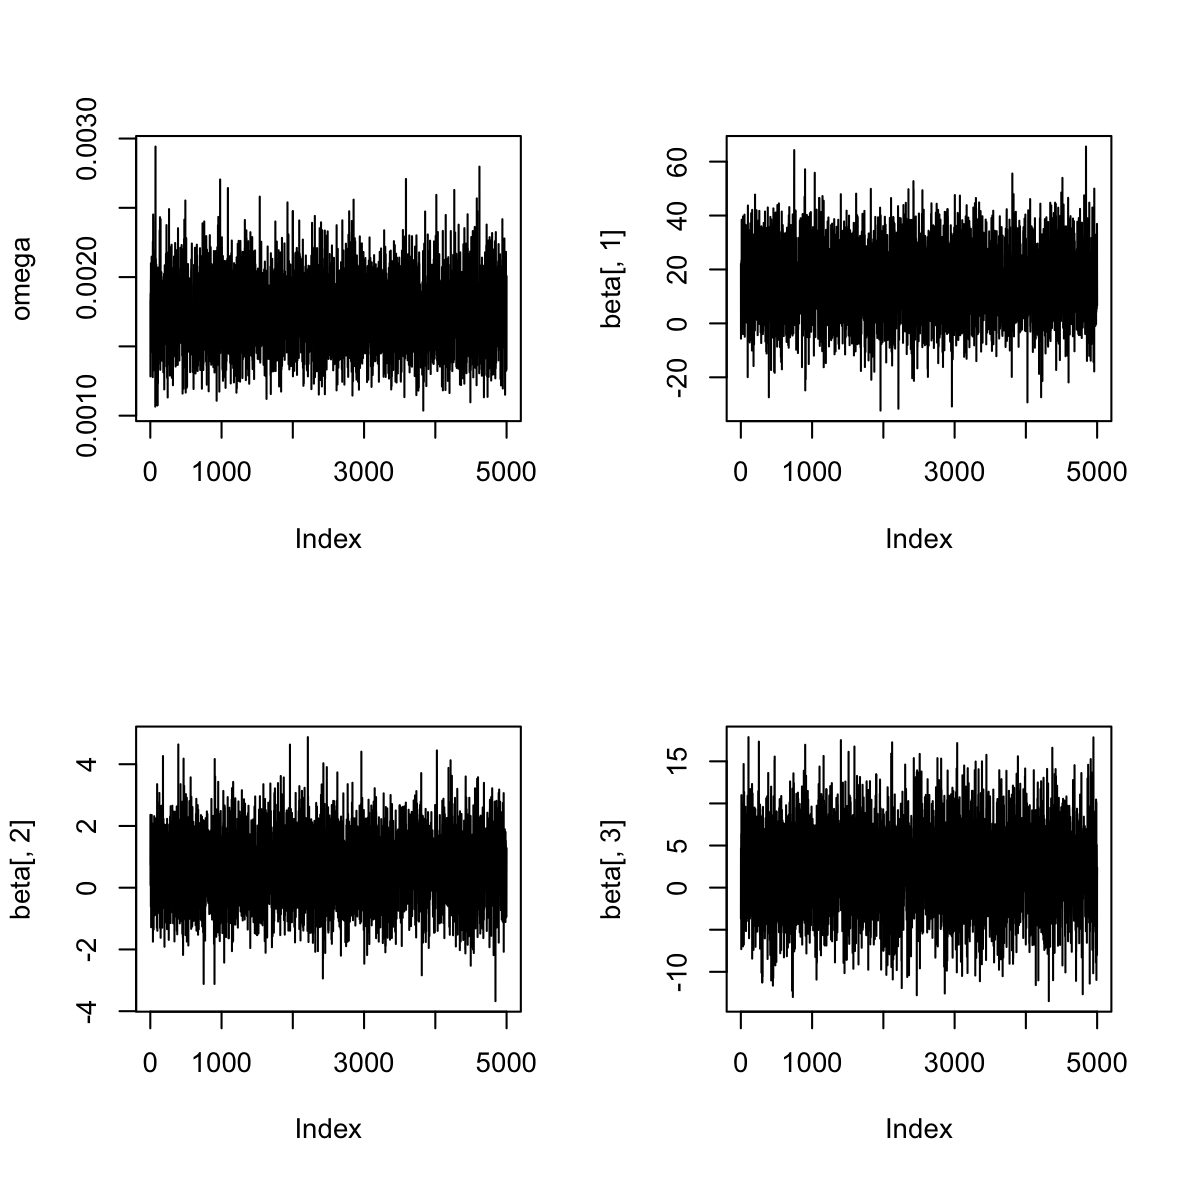
\includegraphics[width=.8\linewidth]{Section2R/Figures/P2_12_Trace.png}
		\caption{Trace plots}
	\end{center}
\end{figure}


\begin{figure}[H]
	\begin{center}
		\begin{subfigure}[h]{0.45\linewidth}
			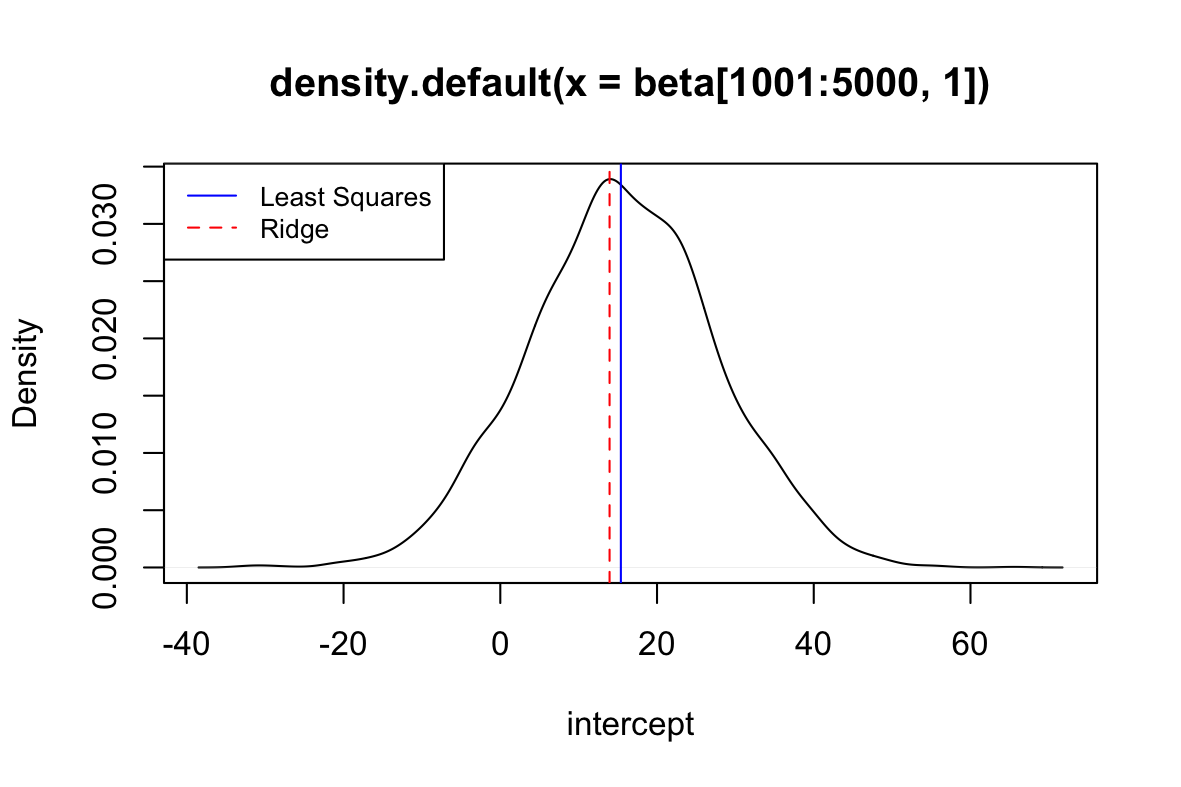
\includegraphics[width=\linewidth]{Section2R/Figures/P2_12_Int.png}
			\caption{Beta Intercept}
		\end{subfigure}
		\begin{subfigure}[h]{0.45\linewidth}
			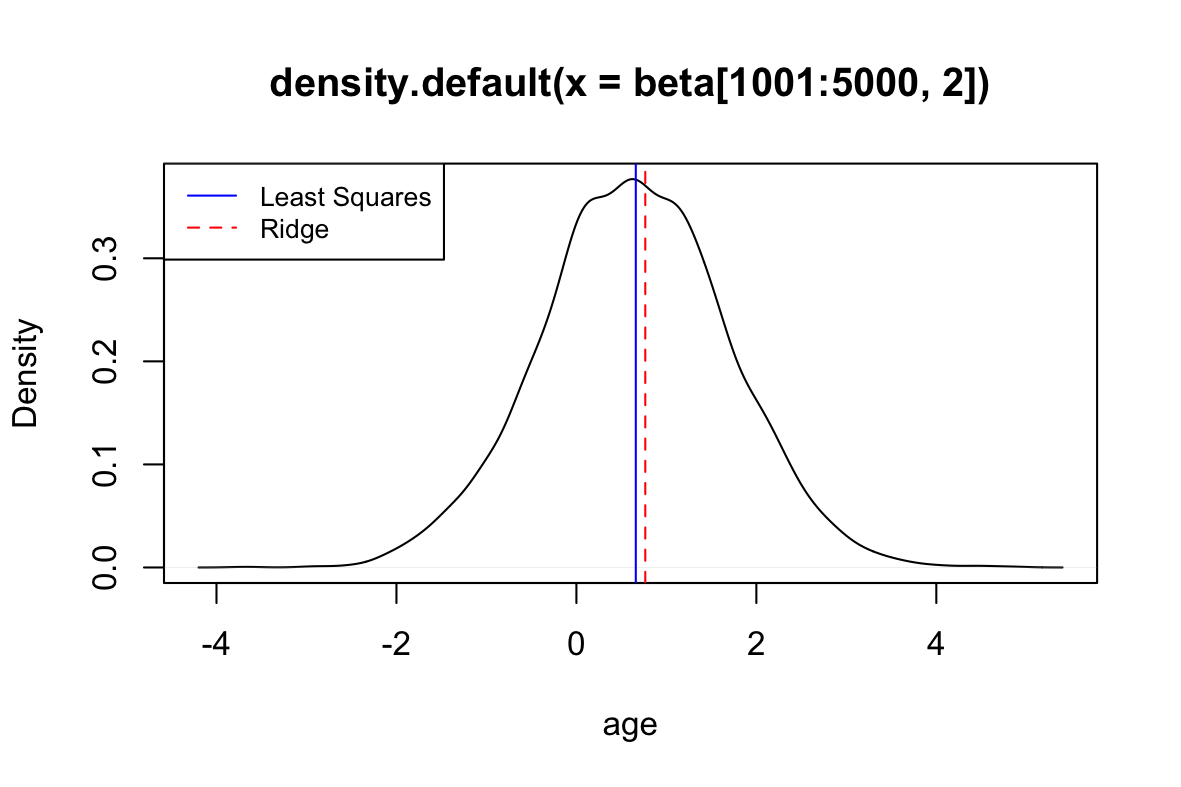
\includegraphics[width=\linewidth]{Section2R/Figures/P2_12_Age.png}
			\caption{Beta Age}
		\end{subfigure}
		\begin{subfigure}[h]{0.45\linewidth}
			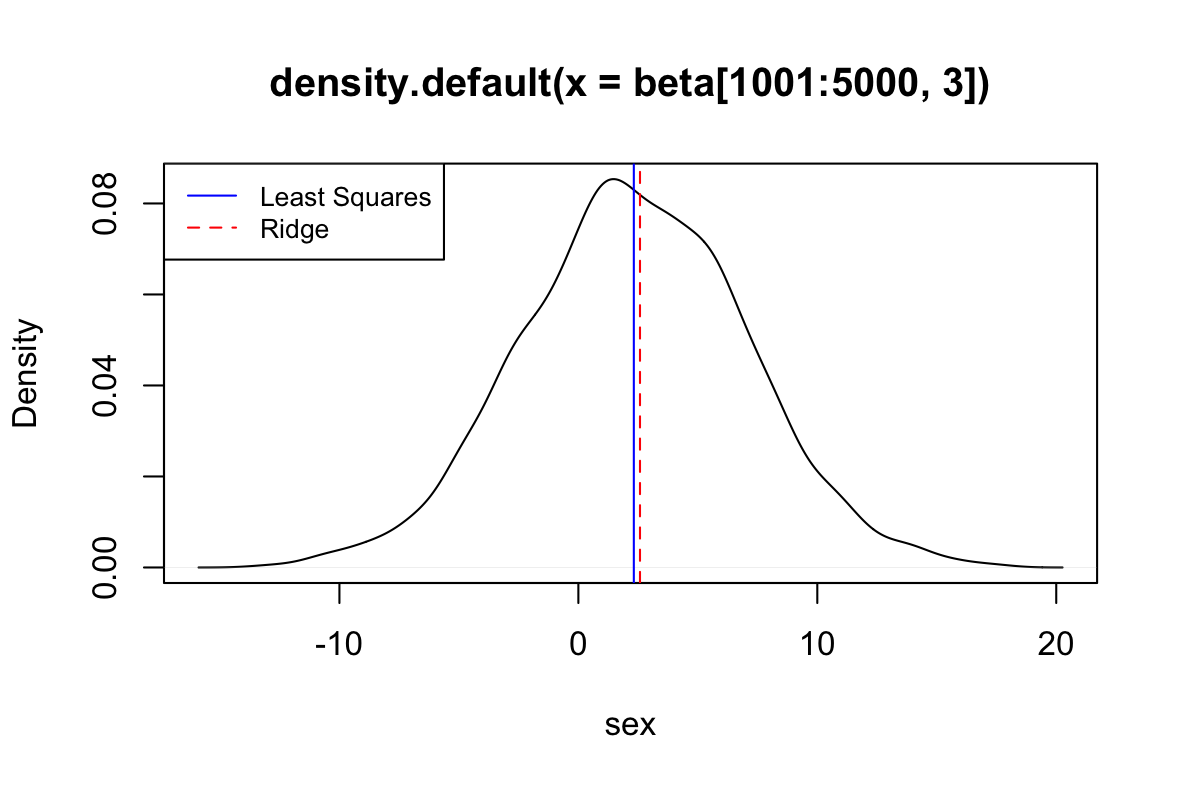
\includegraphics[width=\linewidth]{Section2R/Figures/P2_12_Sex.png}
			\caption{Beta Sex}
		\end{subfigure}
		\caption{Resulting fit comparison}
		\label{fig:Fig2}
	\end{center}
\end{figure}

\color{black}

\section{A hierarchical Gaussian linear model}
The dental dataset has heavier tailed residuals than we would expect under a Gaussian model. We've seen previously that we can model a scaled $t$-distribution using a scale mixture of Gaussians; let's put that into effect here. Concretely, let

$$\begin{aligned}
  \mathbf{y}|\beta,\omega,\Lambda \sim& \mbox{N}(X\beta, (\omega \Lambda)^{-1})\\
  \Lambda =& \mbox{diag}(\lambda_1,\dots, \lambda_n)\\
  \lambda_i \stackrel{\small{iid}}{\sim} \mbox{Gamma}(\tau,\tau)\\
  \beta|\omega \sim& \mbox{N}(\mu, (\omega K)^{-1})\\
  \omega \sim& \mbox{Gamma}(a,b)
\end{aligned}$$

\begin{exercise}
  What is the conditional posterior, $p(\lambda_i|\mathbf{y},\beta, \omega)$?
\end{exercise}

\color{blue}
\textbf{Solution}
$$
p(\lambda_i|\mathbf{y},\beta, \omega) \propto p(y|\omega, \beta, \Lambda)
\propto p(y|\omega, \beta, \Lambda) p(\Lambda) p(\omega, \beta) $$
$ \Lambda $ is independent of $\omega$ and $\beta$
$$
p(\lambda_i|\mathbf{y},\beta, \omega) \propto 
\lambda_i^{\frac{1}{2}} \exp \left\{ - \frac{1}{2} \omega \lambda_i (y_i - x_i \beta)^2 \right\}
\lambda_i^{\tau-1} \exp \left\{-\tau \lambda_i \right\} 
\propto
\lambda_i^{\tau + \frac{1}{2} - 1} \exp \left\{ - \lambda_i \left( \frac{1}{2} \omega  (y_i - x_i \beta)^2 + \tau\right)  \right\}
$$
Which is a Gamma($\tau+\frac{1}{2}, \frac{\omega}{2}  (y_i - x_i \beta)^2 + \tau $)
\color{black}

\begin{exercise}
  Write a Gibbs sampler that alternates between sampling from the conditional posteriors of $\lambda_i$, $\beta$ and $\omega$, and run it for a couple of thousand samplers to fit the model to the dental dataset. 
\end{exercise}

\color{blue}
\textbf{Solution}

Using the script \textit{Section2\_14.R}, 

\color{black}{
	\lstinputlisting[language = R, firstline=23, lastline=63]{Section2R/Section2_14.R}
}

\begin{table}[H]
	\centering
	\caption{Results}
	\label{my-label}
	\begin{tabular}{|l|l|l|l|}
		\hline
		\textbf{} & \textbf{Least Squares} & \textbf{Ridge $ \lambda = 1$} & \textbf{Hierarchical Linear Model} \\ \hline
		Intercept & 15.3857                & 13.9440                     & 15.2847                        \\ \hline
		Age       & 0.6602                 & 0.7656                      & 0.6775                        \\ \hline
		Sex (Male=1)      & 2.3210                 & 2.5793                      & 2.2454                         \\ \hline
	\end{tabular}
\end{table}


\begin{figure}[H]
	\begin{center}
		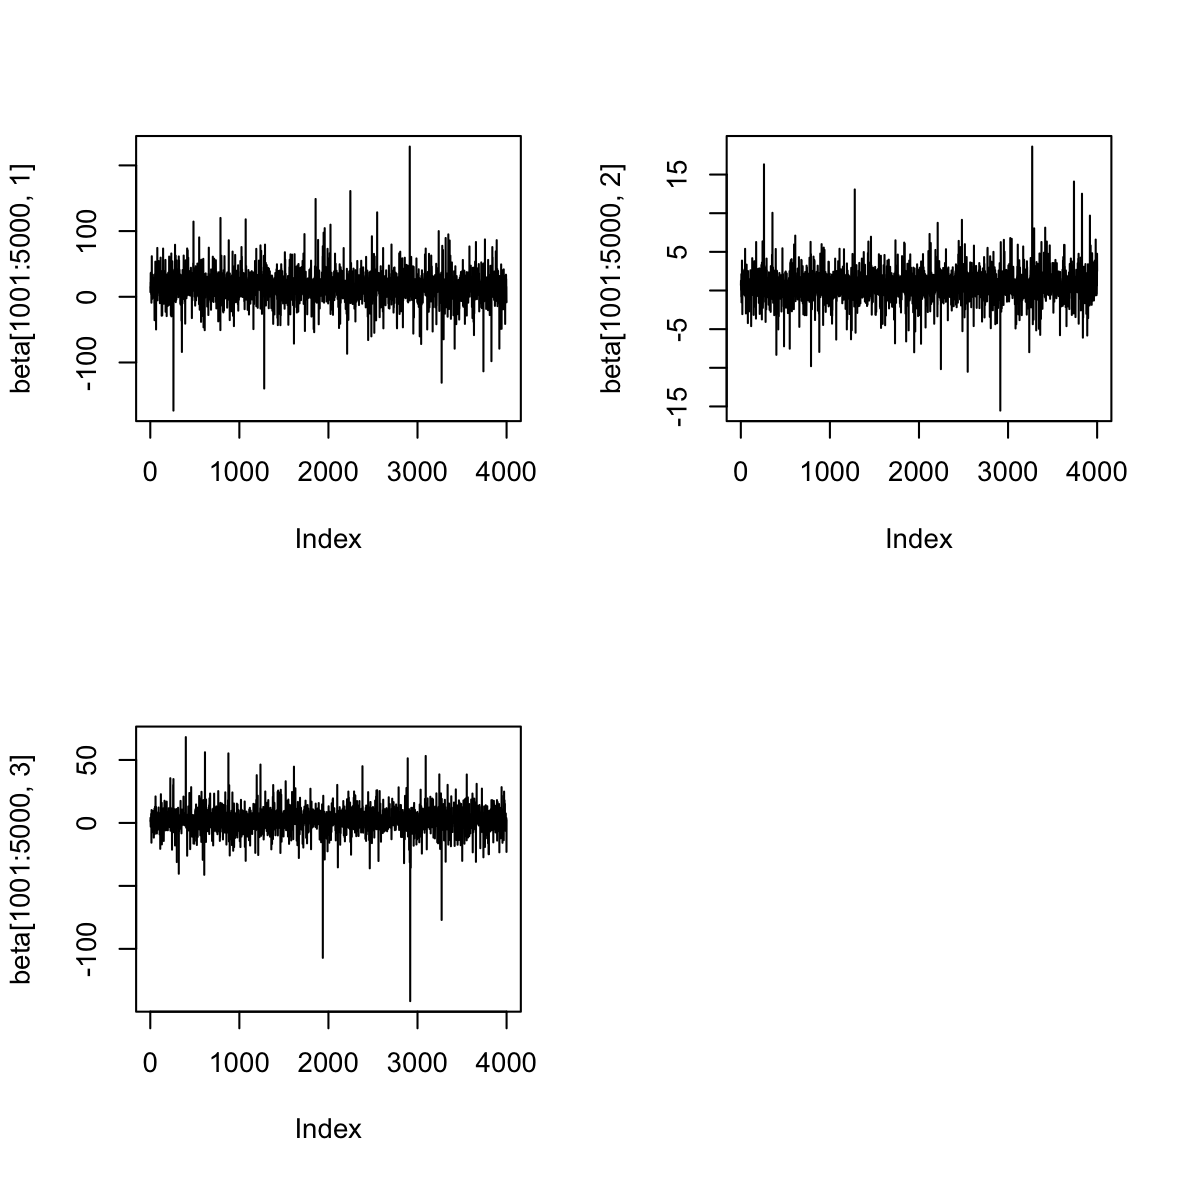
\includegraphics[width=.8\linewidth]{Section2R/Figures/P2_14_Trace.png}
		\caption{Trace plots}
	\end{center}
\end{figure}

\color{black}

\newpage
\begin{exercise}
  Compare the two fits. Does the new fit capture everything we would like? What assumptions is it making? In particular, look at the fit for just male and just female subjects. Suggest ways in which we could modify the model, and for at least one of the suggestions, write an updated Gibbs sampler and run it on your model.
\end{exercise}
  
\color{blue}
\textbf{Solution}

The plot of the residuals of the two models is shown in Figure 2.4. We can observe that the hierarchical model present "fatter tails", this is because the model is more robust with extreme values. 


\begin{figure}[H]
	\begin{center}
		\begin{subfigure}[h]{0.45\linewidth}
			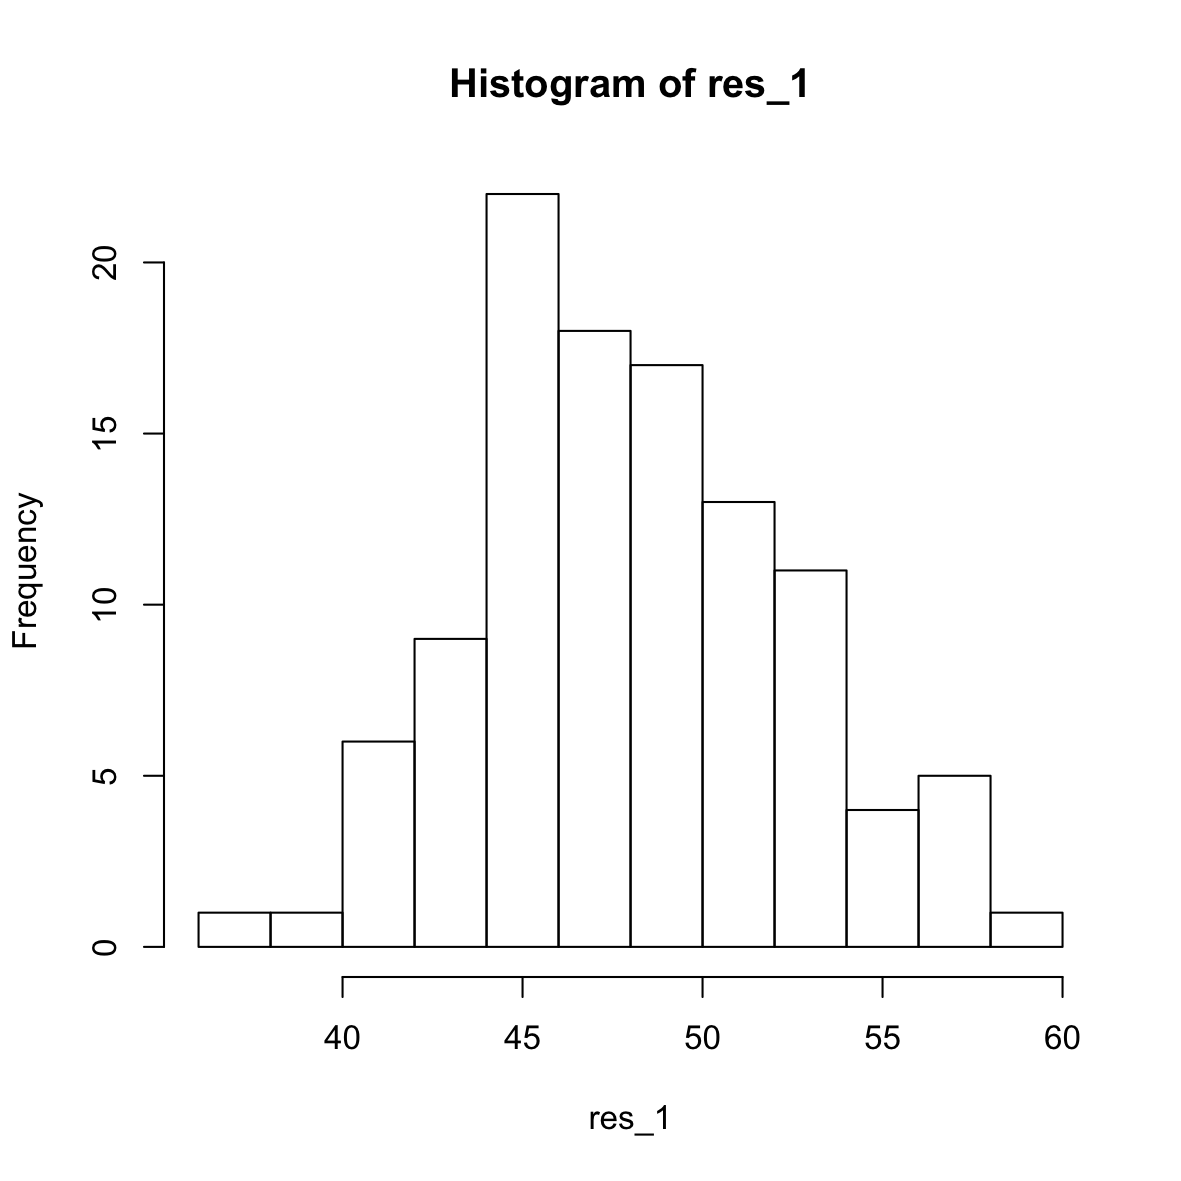
\includegraphics[width=\linewidth]{Section2R/Figures/P2_15_Res1.png}
			\caption{Residuals from the Gaussian Linear Model}
		\end{subfigure}
		\begin{subfigure}[h]{0.45\linewidth}
			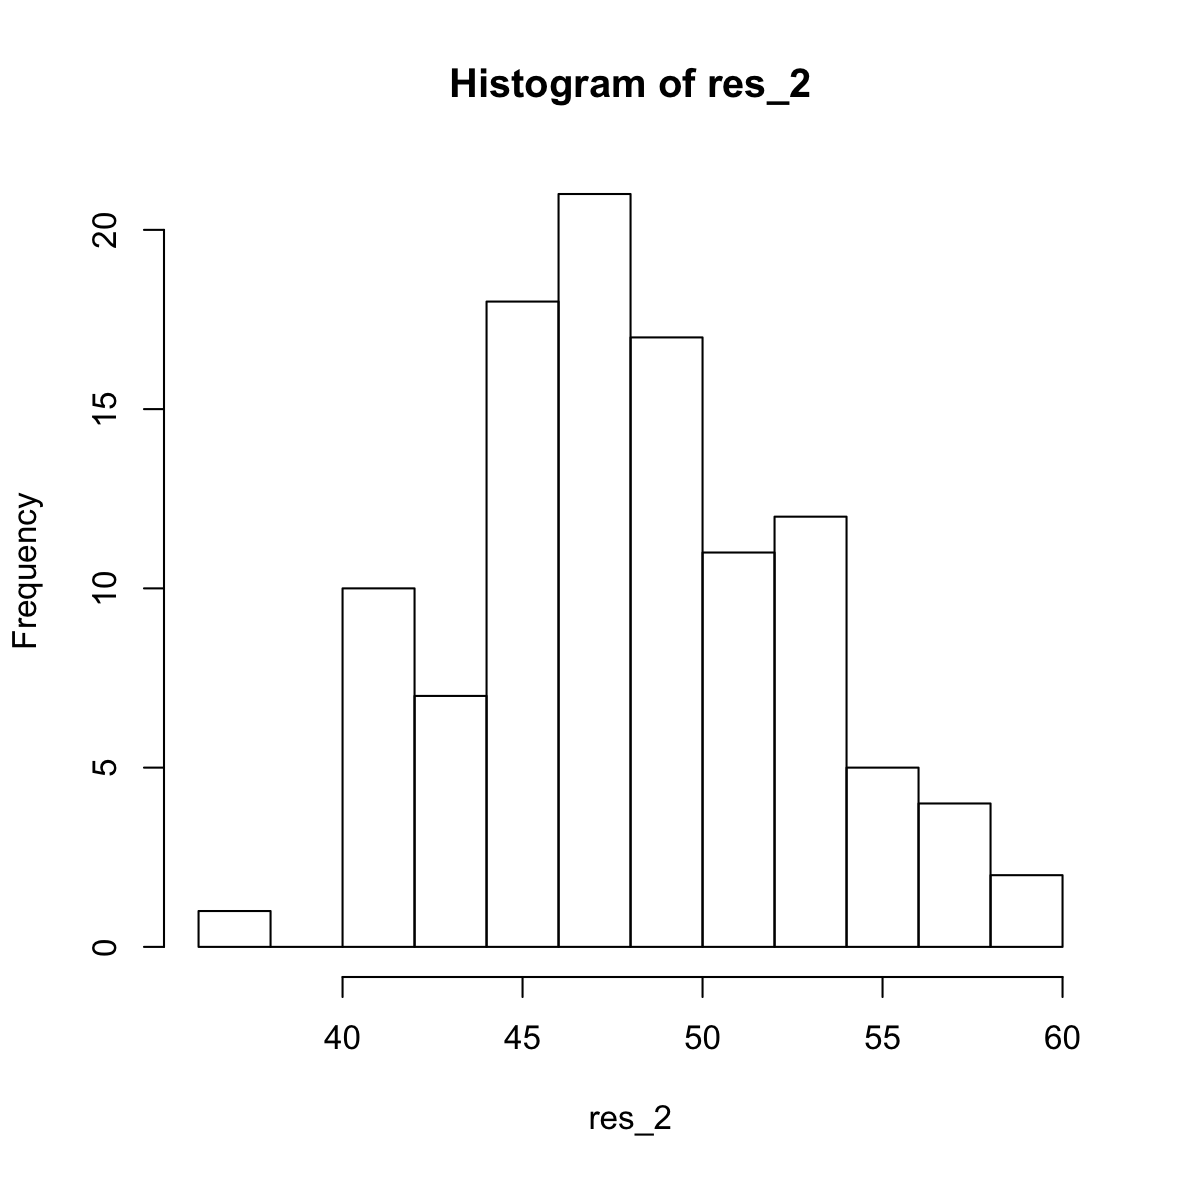
\includegraphics[width=\linewidth]{Section2R/Figures/P2_15_Res2.png}
			\caption{Residuals from the Hierarchical Gaussian Linear Model}
		\end{subfigure}
		\caption{Residuals plot}
		\label{fig:Fig2}
	\end{center}
\end{figure}


We can modify the model by adding interaction terms, since the effect on women and on men is different, this can help to improve the model.

 
\color{black}  

\end{document}
